\chapter{Electronic excitations}
\label{chap:electronic}

We call \textit{electronic} excitations those that, at $\lambda_{ir}=0$, arise from $H_{el}$ in (\ref{eq:full-hamiltonian}). This part of the hamiltonian

\begin{equation}\label{eq:Hel} H_{el} = \sum_n \epsilon_n \rho_n + \sum_{ \langle nm \rangle \sigma } t (c_{n \sigma }^\dagger c_{m \sigma } + H.c.) + U\sum_n \rho_{n\downarrow}\rho_{n\uparrow} \end{equation}

can be represented  as a 9x9 matrix:

\begin{equation}\label{eq:Hel-matrix} \left( \begin{array}{ccccccccc} 
U+2\epsilon &\;\;t\;\;&\;\;0\;\;&\;\;t\;\;&0&\;\;0\;\;&\;\;0\;\;&\;\;0\;\;&0 \\
t&0&t&0&t&0&0&0&0 \\
0&t&2\epsilon &0&0&t&0&0&0 \\
t&0&0&0&t&0&t&0&0 \\
0&t&0&t&U-2\epsilon &t&0&t&0 \\
0&0&t&0&t&0&0&0&t \\
0&0&0&t&0&0&2\epsilon &t&0 \\
0&0&0&0&t&0&t&0&t \\
0&0&0&0&0&t&0&t&U+2\epsilon  \end{array} \right)\end{equation}

and easily diagonalized to see that its first excited state has an energy of ~1376 cm$^{-1}$ above the  ground state.

\begin{figure}
  \centering
  % GNUPLOT: LaTeX picture with Postscript
\begingroup
  \makeatletter
  \providecommand\color[2][]{%
    \GenericError{(gnuplot) \space\space\space\@spaces}{%
      Package color not loaded in conjunction with
      terminal option `colourtext'%
    }{See the gnuplot documentation for explanation.%
    }{Either use 'blacktext' in gnuplot or load the package
      color.sty in LaTeX.}%
    \renewcommand\color[2][]{}%
  }%
  \providecommand\includegraphics[2][]{%
    \GenericError{(gnuplot) \space\space\space\@spaces}{%
      Package graphicx or graphics not loaded%
    }{See the gnuplot documentation for explanation.%
    }{The gnuplot epslatex terminal needs graphicx.sty or graphics.sty.}%
    \renewcommand\includegraphics[2][]{}%
  }%
  \providecommand\rotatebox[2]{#2}%
  \@ifundefined{ifGPcolor}{%
    \newif\ifGPcolor
    \GPcolortrue
  }{}%
  \@ifundefined{ifGPblacktext}{%
    \newif\ifGPblacktext
    \GPblacktextfalse
  }{}%
  % define a \g@addto@macro without @ in the name:
  \let\gplgaddtomacro\g@addto@macro
  % define empty templates for all commands taking text:
  \gdef\gplbacktext{}%
  \gdef\gplfronttext{}%
  \makeatother
  \ifGPblacktext
    % no textcolor at all
    \def\colorrgb#1{}%
    \def\colorgray#1{}%
  \else
    % gray or color?
    \ifGPcolor
      \def\colorrgb#1{\color[rgb]{#1}}%
      \def\colorgray#1{\color[gray]{#1}}%
      \expandafter\def\csname LTw\endcsname{\color{white}}%
      \expandafter\def\csname LTb\endcsname{\color{black}}%
      \expandafter\def\csname LTa\endcsname{\color{black}}%
      \expandafter\def\csname LT0\endcsname{\color[rgb]{1,0,0}}%
      \expandafter\def\csname LT1\endcsname{\color[rgb]{0,1,0}}%
      \expandafter\def\csname LT2\endcsname{\color[rgb]{0,0,1}}%
      \expandafter\def\csname LT3\endcsname{\color[rgb]{1,0,1}}%
      \expandafter\def\csname LT4\endcsname{\color[rgb]{0,1,1}}%
      \expandafter\def\csname LT5\endcsname{\color[rgb]{1,1,0}}%
      \expandafter\def\csname LT6\endcsname{\color[rgb]{0,0,0}}%
      \expandafter\def\csname LT7\endcsname{\color[rgb]{1,0.3,0}}%
      \expandafter\def\csname LT8\endcsname{\color[rgb]{0.5,0.5,0.5}}%
    \else
      % gray
      \def\colorrgb#1{\color{black}}%
      \def\colorgray#1{\color[gray]{#1}}%
      \expandafter\def\csname LTw\endcsname{\color{white}}%
      \expandafter\def\csname LTb\endcsname{\color{black}}%
      \expandafter\def\csname LTa\endcsname{\color{black}}%
      \expandafter\def\csname LT0\endcsname{\color{black}}%
      \expandafter\def\csname LT1\endcsname{\color{black}}%
      \expandafter\def\csname LT2\endcsname{\color{black}}%
      \expandafter\def\csname LT3\endcsname{\color{black}}%
      \expandafter\def\csname LT4\endcsname{\color{black}}%
      \expandafter\def\csname LT5\endcsname{\color{black}}%
      \expandafter\def\csname LT6\endcsname{\color{black}}%
      \expandafter\def\csname LT7\endcsname{\color{black}}%
      \expandafter\def\csname LT8\endcsname{\color{black}}%
    \fi
  \fi
  \setlength{\unitlength}{0.0500bp}%
  \begin{picture}(6802.00,4534.00)%
    \gplgaddtomacro\gplbacktext{%
      \colorrgb{0.31,0.31,0.31}%
      \put(1210,751){\makebox(0,0)[r]{\strut{}\scriptsize 1000}}%
      \colorrgb{0.31,0.31,0.31}%
      \put(1210,1631){\makebox(0,0)[r]{\strut{}\scriptsize 1250}}%
      \colorrgb{0.31,0.31,0.31}%
      \put(1210,2510){\makebox(0,0)[r]{\strut{}\scriptsize 1500}}%
      \colorrgb{0.31,0.31,0.31}%
      \put(1210,3390){\makebox(0,0)[r]{\strut{}\scriptsize 1750}}%
      \colorrgb{0.31,0.31,0.31}%
      \put(1210,4269){\makebox(0,0)[r]{\strut{}\scriptsize 2000}}%
      \colorrgb{0.31,0.31,0.31}%
      \put(1389,484){\makebox(0,0){\strut{}\scriptsize 0}}%
      \colorrgb{0.31,0.31,0.31}%
      \put(1790,484){\makebox(0,0){\strut{}\scriptsize 0.02}}%
      \colorrgb{0.31,0.31,0.31}%
      \put(2192,484){\makebox(0,0){\strut{}\scriptsize 0.04}}%
      \colorrgb{0.31,0.31,0.31}%
      \put(2593,484){\makebox(0,0){\strut{}\scriptsize 0.06}}%
      \colorrgb{0.31,0.31,0.31}%
      \put(2994,484){\makebox(0,0){\strut{}\scriptsize 0.08}}%
      \colorrgb{0.31,0.31,0.31}%
      \put(3395,484){\makebox(0,0){\strut{}\scriptsize 0.1}}%
      \colorrgb{0.31,0.31,0.31}%
      \put(3797,484){\makebox(0,0){\strut{}\scriptsize 0.12}}%
      \colorrgb{0.31,0.31,0.31}%
      \put(4198,484){\makebox(0,0){\strut{}\scriptsize 0.14}}%
      \colorrgb{0.31,0.31,0.31}%
      \put(4599,484){\makebox(0,0){\strut{}\scriptsize 0.16}}%
      \colorrgb{0.31,0.31,0.31}%
      \put(5001,484){\makebox(0,0){\strut{}\scriptsize 0.18}}%
      \colorrgb{0.31,0.31,0.31}%
      \put(5402,484){\makebox(0,0){\strut{}\scriptsize 0.2}}%
      \colorrgb{0.31,0.31,0.31}%
      \put(5803,484){\makebox(0,0){\strut{}\scriptsize 0.22}}%
      \colorrgb{0.31,0.31,0.31}%
      \put(6204,484){\makebox(0,0){\strut{}\scriptsize 0.24}}%
      \csname LTb\endcsname%
      \put(176,2510){\rotatebox{-270}{\makebox(0,0){\strut{}$\omega_i$ (cm$^{-1}$)}}}%
      \put(3897,154){\makebox(0,0){\strut{}$\lambda_{ir}$ (eV)}}%
      \put(3997,3988){\makebox(0,0)[l]{\strut{}\scriptsize$\lambda_{ir}=0.1263$}}%
    }%
    \gplgaddtomacro\gplfronttext{%
    }%
    \gplbacktext
    \put(0,0){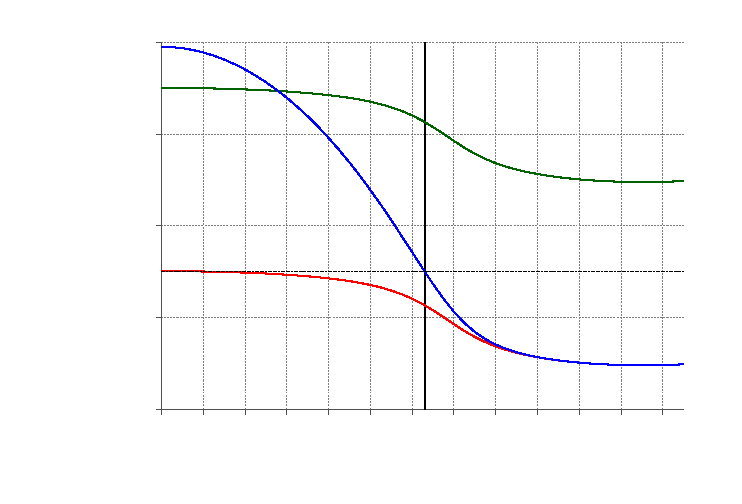
\includegraphics{images/electrSpectra}}%
    \gplfronttext
  \end{picture}%
\endgroup

  \caption[Energy of the electronic excitations as function of $\lambda_{ir}$.]
  {Energy of the electronic excitations as function of $\lambda_{ir}$. 
    The red line corresponds to an electronic excitation with zero phonons, the blue line with one infrared phonon and the green line with one Raman phonon.
    The vertical line is placed at the relevant value $\lambda_{ir}=0.1263$ eV.}
  \label{fig:electrSpectra}
\end{figure}

\section{Projection into definite electronic occupation states}

Since we are using basis states with definite electron occupancy, from the eigenvectors of the (\ref{eq:Hel-matrix}) matrix we can directly see the projections into definite electronic occupation states. The following table summarizes those values omitting equivalent basis states:

\noindent\begin{tabular}{| c | c | c | c | c | c | c | c | c | c |}
\hline
Energy (cm$^{-1}$) & 0.0 & 1376.42 & 3825.49 & 4325.12 & 14897.84 & 15329.82 & 53933.30 & 69272.75 & 69309.3 \\
\hline
$\uparrow \downarrow \ - \ -$ & 0.00276 & 0.00000 & 0.00382 & 0.00000 & 0.00090 & 0.00000 & 0.00179 & 0.49618 & 0.49455 \\
$\uparrow\  \downarrow \ -$ & 0.20130 & 0.19717 & 0.24809 & 0.25000 & 0.04045 & 0.05283 & 0.00606 & 0.00191 & 0.00219 \\
$\uparrow \ - \ \downarrow$ & 0.08522 & 0.10566 & 0.00000 & 0.00000 & 0.41451 & 0.39434 & 0.00023 & 0.00000 & 0.00000 \\
$ - \ \uparrow \downarrow \ -$ & 0.01884 & 0.00000 & 0.00000 & 0.00000 & 0.00736 & 0.00000 & 0.97174 & 0.00000 & 0.00205 \\
\hline
\end{tabular}

We noticed\cite{GarciaSaraviaOrtizdeMontellano2013} that, for the first \textit{electronic} excitation, the projection into states with an electron in each oxygen decreases with an increasing $\lambda_{ir}$ suggesting partial charge localization.

\section{Projection into phonon coordinates}

\begin{figure}[ht!]
\centering
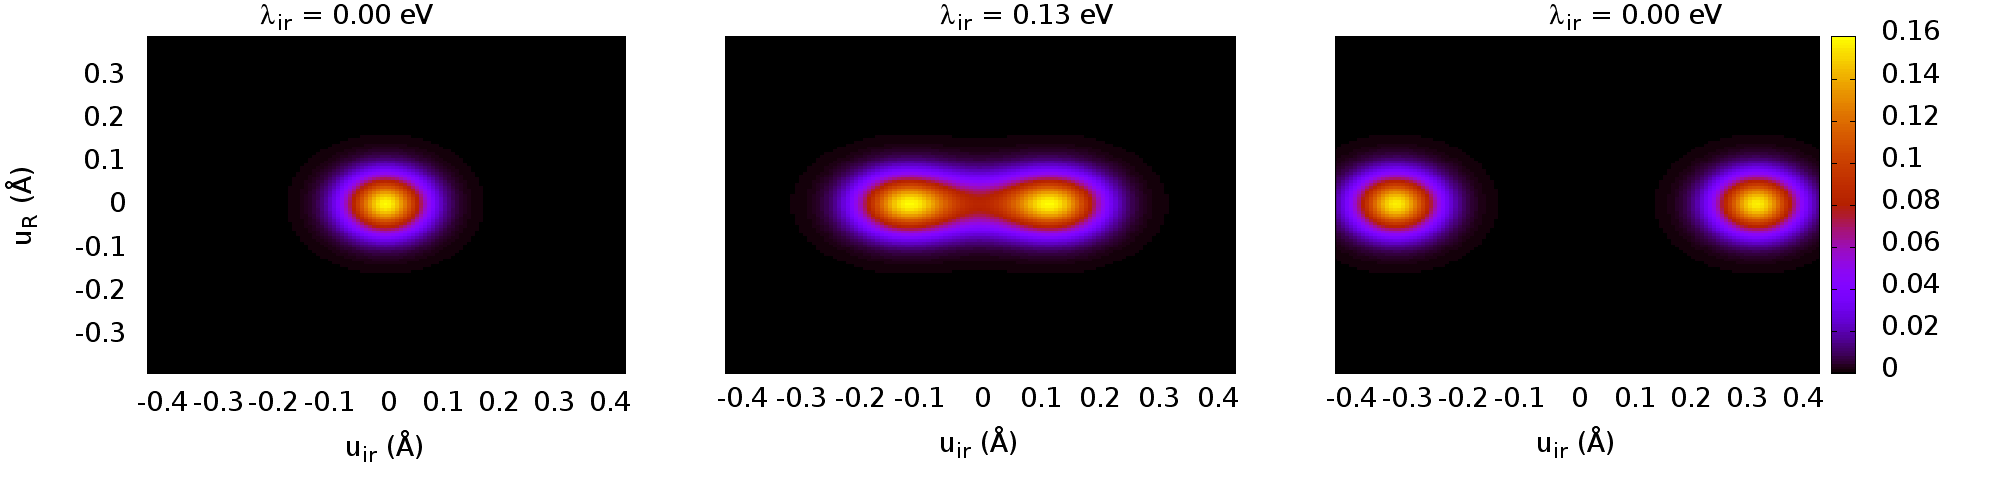
\includegraphics[width=0.8\textwidth]{images/ph-electronic.png}
\caption{Electronic state projected into phonon coordinates for three representative electron-lattice coupling ($\lambda_{ir}$) values.}
\label{fig:ph-electronic.png}
\end{figure}

\section{Isotopic shift}

\begin{figure}[ht!]
\centering
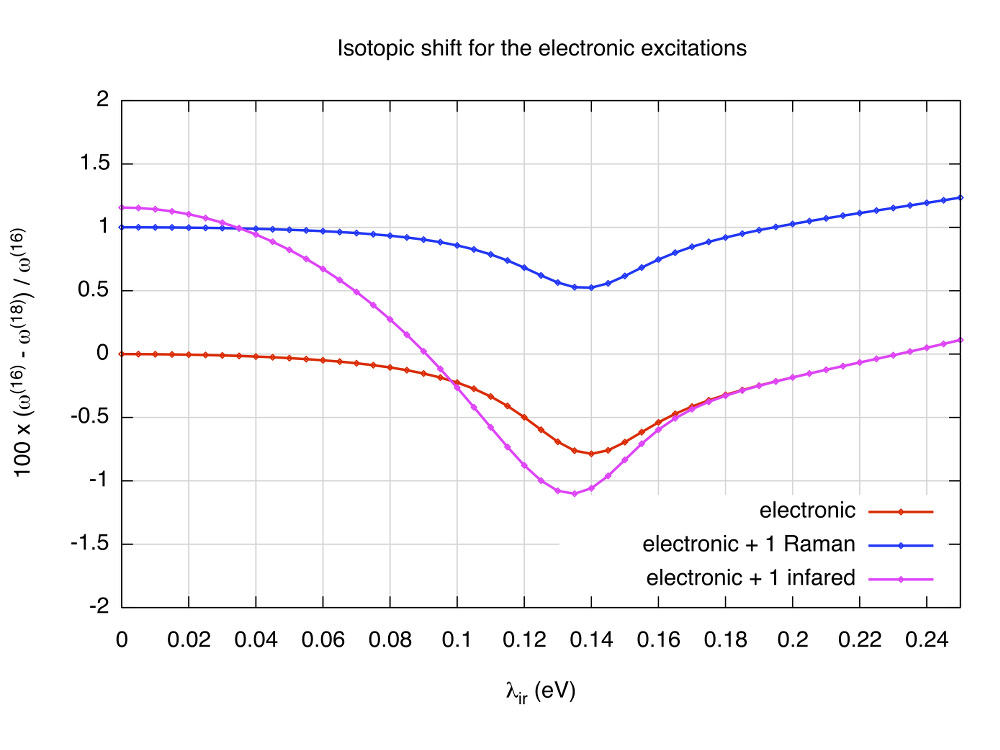
\includegraphics[width=0.8\textwidth]{images/isot-el.jpg}
\caption{Isotopic shift for the electronic state.}
\label{fig:isot-el}
\end{figure}

